\documentclass[border=3pt,tikz]{standalone}
\usepackage{amsmath}
\usetikzlibrary{calc}
\usetikzlibrary{arrows.meta} % for arrow size
\begin{document}
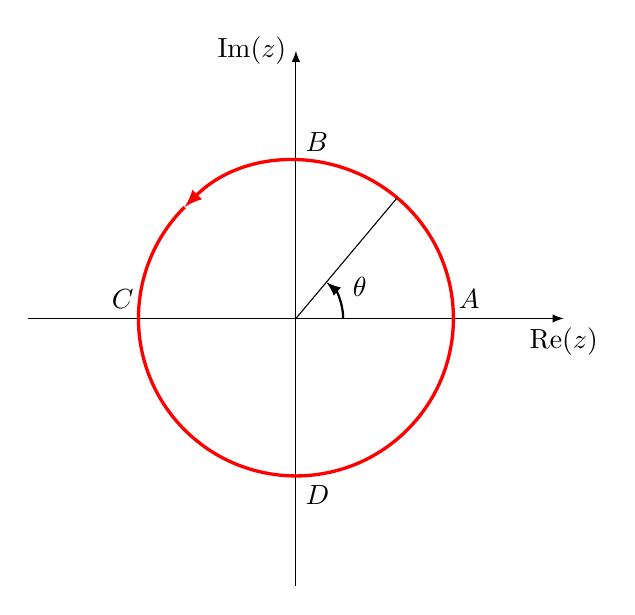
\begin{tikzpicture}[scale=2]
    \usetikzlibrary {arrows.meta}
    \usetikzlibrary {calc}
    
    \coordinate (z0) at (0, 0);
    \coordinate (z1) at ({cos(50)}, {sin(50)});
    \coordinate (zp) at (2.201, 1.497);
    \draw [-latex] (-1.7, 0) -- (1.7, 0) node[below] {Re$(z)$};
    \draw [-latex] (0, -1.7) -- (0, 1.7) node[left] {Im$(z)$};
    
    
    \draw[red, very thick, -latex,] ({cos(135)}, {sin(135)}) arc (135:495:1);
    \draw[thick, -latex] (0.3, 0) arc (0:50:0.3);
    \node [right] at (0.3, 0.2) {$\theta$};
    \node [above] at(1.1, 0.0) {$A$};
    \node [above right] at(0.0, 1.0) {$B$};
    \node [above] at(-1.1, 0) {$C$};
    \node [below right] at(0.0, -1.0) {$D$};
    \draw[] (z0) -- (z1);
    
    \end{tikzpicture}
\end{document}